\documentclass[a4paper,11pt]{report}

\usepackage[utf8]{inputenc}
\usepackage[T1]{fontenc}
\usepackage[francais]{babel}

\usepackage{graphicx}
\usepackage{tabularx}
\usepackage{arydshln}

\usepackage{pdflscape}
\usepackage{pdfpages}
\usepackage{chronology}
%%%%%%%%%%%%%% http://tex.stackexchange.com/questions/171782/error-with-chronology-and-babel-packages-paragraph-ended-before-pgffornex %%%%%%%%%%%%%%
\let\CHRONOLOGY\chronology
\let\endCHRONOLOGY\endchronology
\def\chronology{\shorthandoff{;}\CHRONOLOGY}
\def\endchronology{\endCHRONOLOGY\shorthandon{;}}
%%%%%%%%%%%%%%%%%%%%%%%%%%%%%%%%%%%%%%%%%%%%%%%%%%%%%%%%
\usepackage{fullpage}

\setcounter{secnumdepth}{3}

\title{Evalens -- Analyse}
\date{}

\begin{document}
\maketitle
\tableofcontents

\chapter{Lexique}

\subsection{Doyen}

\subsection{Gestionnaire de campagne}
Entité pouvant être composée de plusieurs personnes.

\subsection{Commision pédagogique facultaire}
\subsubsection{Membre}
\subsubsection{Président}

\subsection{Étudiant}

\subsection{Enseignant}

\subsection{Cellule de communication universitaire}

\subsection{Unité d'enseignement}

\subsection{Campagne}

\subsection{Calendrier}

\subsection{Période}
Intervalle de temps ayant une date et une heure de début et de fin.

\subsection{Département de support aux activités académiques (DSAA)}

\chapter{Cas d'utilisation}
\begin{figure}[ht]
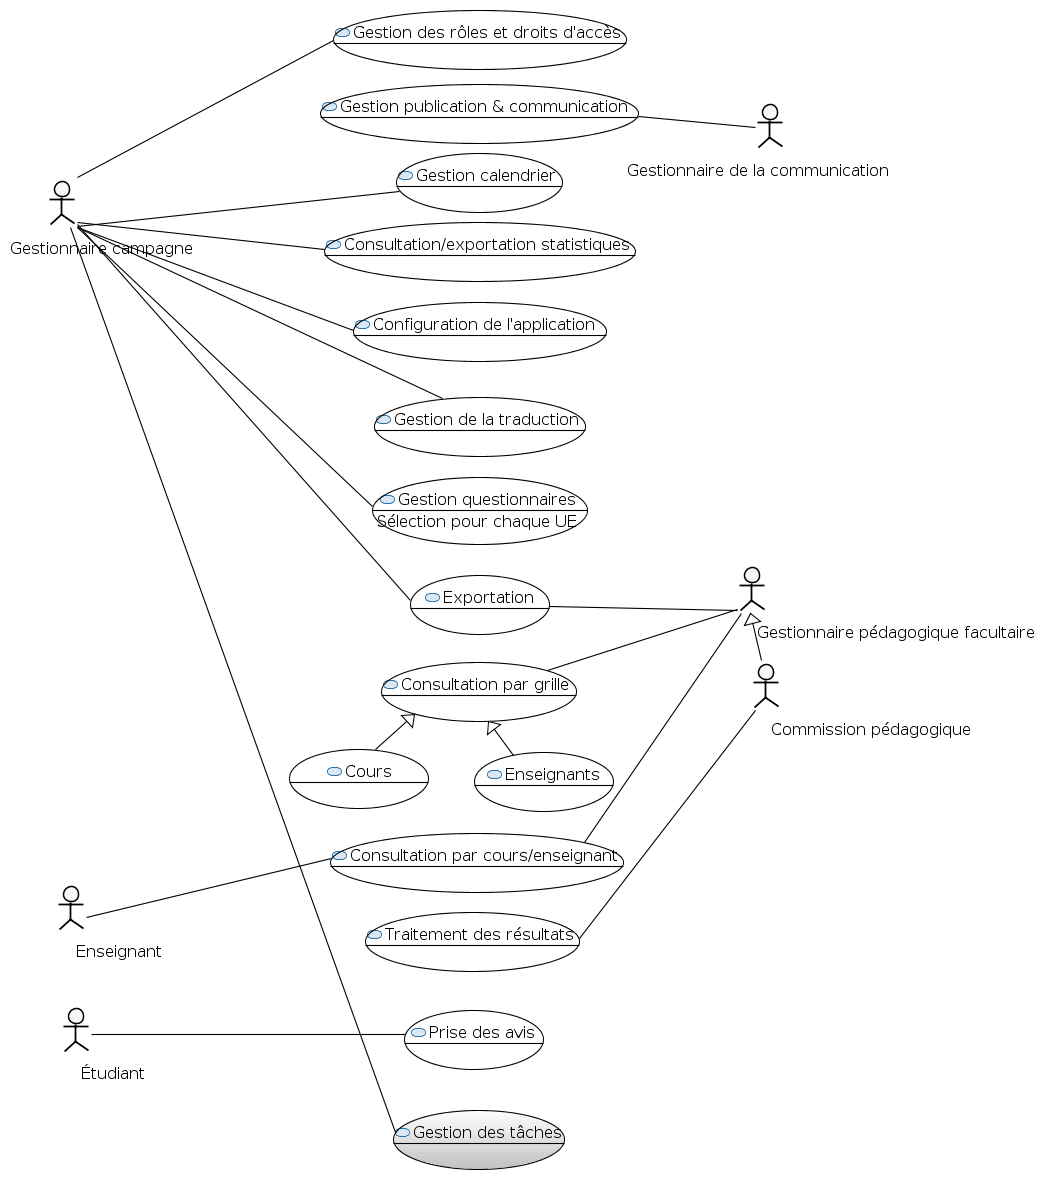
\includegraphics[width=\linewidth]{UseCase_Diagram.PNG}
\caption{Diagramme des cas d'utilisation}
\label{fig:usecase-diag}
\end{figure}

\section{Évaluation des enseignements}






%%%%%%%%%%%%%%%%%%%%%%%%%%%%%%%%%%%%%%%%%%%%%%%%%%%%%%%%%%%%%%%
%      GESTION DES RÔLES ET DES DROITS D'ACCÈS
%%%%%%%%%%%%%%%%%%%%%%%%%%%%%%%%%%%%%%%%%%%%%%%%%%%%%%%%%%%%%%%
\subsection{Gestion des rôles et des droits d'accès}
Chaque utilisateur a un rôle et des droits d'accès différents.

\begin{table}[ht]
\begin{tabularx}{\textwidth}{|X|l|} \hline
Rôle & Droits d'accès \\ \hline
Gestionnaire des rôles et droits d'accès & \\ \hline
Gestionnaire des publications et de la communication & \\ \hline
Configuration de l'application & \\ \hline
Gestionnaire de la traduction & \\ \hline
Gestionnaire des questionnaires & \\ \hline
DAF & \\ \hline
Président de la com péd & \\ \hline
Gestionnaire de calendrier & \\ \hline

\end{tabularx}
\caption{Rôle et droits d'accès des différents utilisateurs du système. «~com. péd.~» est l'abbréviation de «~commission pédagogique~».}
\label{tab:role-droit}
\end{table}

Certains rôles et droits d'accès peuvent être amenés à évoluer, et d'autres pourraient être ajoutés par la suite.






%%%%%%%%%%%%%%%%%%%%%%%%%%%%%%%%%%%%%%%%%%%%%%%%%%%%%%%%%%%%%%%
%      GESTION DES PUBLICATIONS ET DE LA COMMUNICATION
%%%%%%%%%%%%%%%%%%%%%%%%%%%%%%%%%%%%%%%%%%%%%%%%%%%%%%%%%%%%%%%
\subsection{Gestion des publications et de la communication}
La gestion des publications et de la campagne a pour objectif de maintenir au courant la communauté universitaire du statut de la campagne d'évaluation.
Cette communication est assurée par un gestion de la communication.
Le corps de la communication se base sur un modèle pouvant être modifié selon les besoins.

\noindent Les informations suivantes doivent être communiquées~:
\begin{itemize}
	\item le calendrier d'ouverture de la campagne d'évaluation
	\item les rapports statistiques (à la commission pédagogique)
	\item invitation\footnote{Est-ce lui qui s'occupe du contenu des invitation à la prise d'avis, ainsi que du contenu des rappels~?} ?
	\item rappel ?
	\item Disponibilité des résultats ?
\end{itemize}

Les communications peuvent prendre la forme d'un simple courriel ou d'un fichier \texttt{pdf} devant être mis à disposition des systèmes et/ou personnes concernés.


\subsubsection{Processus}
\paragraph{Élément déclencheur}~\newline{}

% \paragraph{Planification}~\newline{}

% \begin{tabularx}{\linewidth}{|X|X|X|} \hline
% Fréquence du processus & Début & Fin \\ \hline
% &  &  \\ \hline
% \end{tabularx}

\paragraph{Data}~\newline{}

\begin{tabularx}{\linewidth}{|X|X|} \hline
Data In & Data Out \\ \hline
 & \\ \hline
\end{tabularx}

\paragraph{Data In du processus}~\newline{}

\begin{tabularx}{\linewidth}{|X|X|X|X|} \hline
Data & Type & Source & Destiné à l'acteur \\ \hline

\end{tabularx}

\paragraph{Data Out du processus}~\newline{}

\begin{tabularx}{\linewidth}{|X|X|X|X|} \hline
Data & Type & État & Destination \\ \hline
Calendrier d'ouverture de campagne & Document électronique & Complet & Communauté universitaire\footnote{À véfifier, car « calendrier ouverture application evalens » est indiqué comme « interne ».} \\
Rapport statistique & Document électronique & Complet & Commission pédagogique facultaire \\ \hline
\end{tabularx}

\paragraph{Acteurs}~\newline{}

\begin{tabularx}{\linewidth}{|X|X|X|X|X|} \hline
Nom & Rôle & Actions & Data In & Data Out \\ \hline 
Gestionnaire de communication & Gestion de la communication & Communique les informations reprises dans cette section à leurs destinataires & ?? & 
	\begin{itemize} 
		\item Calendrier d'ouverture de campagne d'évaluation
		\item Rapport statistique
	\end{itemize}
\\ \hline
\end{tabularx}










%%%%%%%%%%%%%%%%%%%%%%%%%%%%%%%%%%%%%%%%%%%%%%%%%%%%%%%%%%%%%%%
%      GESTION DU CALENDRIER
%%%%%%%%%%%%%%%%%%%%%%%%%%%%%%%%%%%%%%%%%%%%%%%%%%%%%%%%%%%%%%%
\subsection{Gestion du calendrier}
La gestion du calendrier est une étape nécessaire à une campagne~; elle permet de définir les périodes de validité de certaines activités ainsi que les dates de planification des tâches, potentiellement par faculté.
Cette gestion permet de déclarer une période de suspension pour toute période définie en cas de besoin.

\noindent Elle est prise en charge par le gestionnaire de campagne.

\noindent Parmi ces dates et périodes, on trouve~:
\begin{itemize}
	\item Invitation à la prise d'avis~: date et heure à laquelle le mail d'invitation à la prise d'avis est envoyé aux étudiants.
	\item Rappel à la prise d'avis~: date et heure à laquelle le mail de rappel de prise d'avis est envoyé aux participants qui n'ont pas rempli certains critères (exemple~: participants ayant répondu à moins de 80~\% des questions).
	\item Prise d'avis~: période durant laquelle les étudiants ont accès aux questionnaires et peuvent les remplir.
	\item Traitement des résultats~: période durant laquelle la commission pédagogique a accès au traitement des résultats. La commission a aussi l'opportunité de consulter les résultats à partir du début de cette période, dès lors que le traitement est terminé.
	\item Consultation des résultats par les enseignants~: date à partir de laquelle les enseignants ont accès aux résultats de la campagne.
	\item Consultation des résultats par grille~: date à partir de laquelle les résultats par grille sont accessibles par un ensemble de rôle.
\end{itemize}
~\newline{}

La constitution du calendrier est régie par les règles et contraintes suivantes~:
\begin{itemize}
	\item Chaque date et période déclarée doit être liée à une campagne.
	\item La période de prise d'avis doit être incluse dans la période de la campagne.
	\item La période de prise d'avis doit durer au moins deux semaines (annexe~\ref{an:regl-cadre}).
	\item La date d'invitation des prises d'avis doit être entérieure à la date de début de la période de prise d'avis.
	\item La date de rappel à la prise d'avis doit être incluse dans la période de prise d'avis.
	\item Le traitement des résultats est suspendu tant qu'une période de prise d'avis est en cours.
	\item La date de consultation des résultats par les enseignants doit être postérieure à la date de fin de la période de traitement des résultats.
\end{itemize}


% \begin{landscape}
\subsubsection{Processus}
\paragraph{Élément déclencheur}~\newline{}

Planification du superviseur pour respecter les décisions du règlement cadre (annexe~\ref{an:regl-cadre}\footnote{Règlement cadre du 02 février 2015 (version 1.1).}).

\paragraph{Planification}~\newline{}

\begin{tabularx}{\linewidth}{|X|X|X|} \hline
Fréquence du processus & Début & Fin \\ \hline
Deux fois par année académique (annexe~\ref{an:regl-cadre})~: & & \\
& & \\
Période 2 & En février après la session d'examens de janvier & deux semaines plus tard \\
& & \\ %\hdashline
Périodes 1 et 3 & En juin après la session d'examens de juin & trois semaines plus tard \\
& après la session d'août & deux semaines plus tard \\ \hline
\end{tabularx}
% Info tirées du "règlement cadre" et du cahier des charges.

\paragraph{Data}~\newline{}

\begin{tabularx}{\linewidth}{|X|X|} \hline
Data In & Data Out \\ \hline
N/A & Périodes composant le calendrier de campagne~:
\begin{itemize}
	\item Période de prise d'avis
	\item Date d'invitation à la prise d'avis
	\item Période de traitement des résultats
	\item Date de consultation des résultats
	\item etc.
\end{itemize}
~\\ \hline
\end{tabularx}

% \paragraph{Data In du processus}
% \begin{tabularx}{\linewidth}{|X|X|X|X|} \hline
% Data & Type & Source & Destiné à l'acteur \\ \hline
% \end{tabularx}

\paragraph{Data Out du processus}~\newline{}

\begin{tabularx}{\linewidth}{|X|X|X|X|} \hline
Data & Type & État & Destination \\ \hline
Calendrier & Base de données & Complet, peut faire l'objet de mises à jour & ?? \\ \hline
\end{tabularx}

\paragraph{Acteurs}~\newline{}

\begin{tabularx}{\linewidth}{|X|X|X|X|X|} \hline
Nom & Rôle & Actions & Data In & Data Out \\ \hline
% Commission pédagogique & 
Superviseur & Gestionnaire de calendrier & Établissement des dates & N/A & Calendrier de la campagne \\ \hline
\end{tabularx}

% \end{landscape}

% \begin{chronology}[1]{2016}{2017}{3em}{\linewidth}%
% \event{\decimaldate{15}{02}{2016}}{three}
% \end{chronology}





%%%%%%%%%%%%%%%%%%%%%%%%%%%%%%%%%%%%%%%%%%%%%%%%%%%%%%%%%%%%%%%
%      CONFIGURATION DE L'APPLICATION
%%%%%%%%%%%%%%%%%%%%%%%%%%%%%%%%%%%%%%%%%%%%%%%%%%%%%%%%%%%%%%%
\subsection{Configuration de l'application}
L'architecture de l'application offre la possibilité au superviseur de modifier la configuration de certains paramètres.

\noindent Ces paramètres font partie de la liste suivante~:
\begin{itemize}
	\item quorum~;
	\item etc.
\end{itemize}





%%%%%%%%%%%%%%%%%%%%%%%%%%%%%%%%%%%%%%%%%%%%%%%%%%%%%%%%%%%%%%%
%      GESTION DE LA TRADUCTION
%%%%%%%%%%%%%%%%%%%%%%%%%%%%%%%%%%%%%%%%%%%%%%%%%%%%%%%%%%%%%%%
\subsection{Gestion de la traduction}
La gestion de la traduction permet de traduire les données de présentation relatives à l'évaluation des enseignements dans une autre langue que le français.
Le superviseur se charge de récupérer l'ensemble des données devant être traduites avant de les confier au DSAA, comme stipulé dans l'annexe~\ref{an:regl-cadre}.
Les données à traduire sont les suivantes~:
\begin{itemize}
	\item Questionnaires
	\item Interfaces utilisateur~:
	\begin{itemize}
		\item L'interface à destination des étudiants doit être traduite, en accord avec le règlement cadre (cf. annexe~\ref{an:regl-cadre}).
		\item Les interfaces à destination des enseignants et des commissions peuvent être traduites.
	\end{itemize}
\end{itemize}

% \begin{landscape}
\subsubsection{Processus}
\paragraph{Élément déclencheur}~\newline{}
Requête de la part du superviseur.

\paragraph{Planification}~\newline{}

\begin{tabularx}{\linewidth}{|X|X|X|} \hline
Fréquence du processus & Début & Fin \\ \hline
Une fois & N/A & Avant la période de prise d'avis \\ \hline
\end{tabularx}

\paragraph{Data}~\newline{}

\begin{tabularx}{\linewidth}{|X|X|} \hline
Data In & Data Out \\ \hline
Questionnaires et textes de l'interface en français & Questionnaires et textes traduits\\ \hline
\end{tabularx}

\paragraph{Data In du processus}~\newline{}

\begin{tabularx}{\linewidth}{|X|X|X|X|} \hline
Data & Type & Source & Destiné à l'acteur \\ \hline
Questionnaires et textes en français & Base de données & Application ? & DSAA\\ \hline
\end{tabularx}

\paragraph{Data Out du processus}~\newline{}

\begin{tabularx}{\linewidth}{|X|X|X|X|} \hline
Data & Type & État & Destination \\ \hline
Questionnaires et textes traduits & Base de données & En cours & Superviseur \\ \hline
\end{tabularx}

\paragraph{Acteurs}~\newline{}

\begin{tabularx}{\linewidth}{|X|X|X|X|X|} \hline
Nom & Rôle & Actions & Data In & Data Out \\ \hline 
Superviseur & Gestionnaire de la traduction & Supervise et confie la traduction des questionnaires et des textes de l'interface au DSAA, en accord avec le règlement cadre~(cf. annexe~\ref{an:regl-cadre}) & Questionnaires et textes en français & Questionnaires et textes traduits \\ 
DSAA & Traduction & Traduit les données qui lui sont communiquées depuis le français & Questionnaires et textes en français & Questionnaires et textes traduits \\ \hline
\end{tabularx}

% \end{landscape}





%%%%%%%%%%%%%%%%%%%%%%%%%%%%%%%%%%%%%%%%%%%%%%%%%%%%%%%%%%%%%%%
%      GESTION DES QUESTIONNAIRES
%%%%%%%%%%%%%%%%%%%%%%%%%%%%%%%%%%%%%%%%%%%%%%%%%%%%%%%%%%%%%%%
\subsection{Gestion des questionnaires}
Lors de chaque campagne, un questionnaire est associé à chaque unité d'enseignement.
Ce questionnaire peut changer d'une campagne à l'autre, mais il doit être possible de retrouver celui correspondant à une campagne donnée.

Cf. règlement cadre Article 5

Au moins un mois avant le début de la période de prise d'avis, le recteur ou le vice-recteur désigné par lui sollicite les enseignants pour vérifier l'exactitude des données liées à leurs unités d'enseignement.







%%%%%%%%%%%%%%%%%%%%%%%%%%%%%%%%%%%%%%%%%%%%%%%%%%%%%%%%%%%%%%%
%      EXPORTATION
%%%%%%%%%%%%%%%%%%%%%%%%%%%%%%%%%%%%%%%%%%%%%%%%%%%%%%%%%%%%%%%
\subsection{Exportation}
Les différentes données accessibles à l'utilisateur doivent pouvoir être exportées en différents formats~:
\begin{itemize}
	\item CSV
	\item PDF
\end{itemize}






%%%%%%%%%%%%%%%%%%%%%%%%%%%%%%%%%%%%%%%%%%%%%%%%%%%%%%%%%%%%%%%
%      CONSULTATION DES RÉSULTATS PAR GRILLES
%%%%%%%%%%%%%%%%%%%%%%%%%%%%%%%%%%%%%%%%%%%%%%%%%%%%%%%%%%%%%%%
\subsection{Consultation des résultats par grilles}






%%%%%%%%%%%%%%%%%%%%%%%%%%%%%%%%%%%%%%%%%%%%%%%%%%%%%%%%%%%%%%%
%      CONSULTATION PAR COURS/ENSEIGNANT
%%%%%%%%%%%%%%%%%%%%%%%%%%%%%%%%%%%%%%%%%%%%%%%%%%%%%%%%%%%%%%%
\subsection{Consultation par cours/enseignant}
Les enseignants ont la possibilité de consulter leurs résultats de deux façons différentes~:
\begin{itemize}
	\item en vue globale rassemblant toutes leurs unités d'enseignement~;
	\item une unité d'enseignement à la fois.
\end{itemize}

Les titulaires des unités d'enseignement peuvent consulter






%%%%%%%%%%%%%%%%%%%%%%%%%%%%%%%%%%%%%%%%%%%%%%%%%%%%%%%%%%%%%%%
%      TRAITEMENT DES RÉSULTATS
%%%%%%%%%%%%%%%%%%%%%%%%%%%%%%%%%%%%%%%%%%%%%%%%%%%%%%%%%%%%%%%
\subsection{Traitement des résultats}






%%%%%%%%%%%%%%%%%%%%%%%%%%%%%%%%%%%%%%%%%%%%%%%%%%%%%%%%%%%%%%%
%      PRISE DES AVIS
%%%%%%%%%%%%%%%%%%%%%%%%%%%%%%%%%%%%%%%%%%%%%%%%%%%%%%%%%%%%%%%
\subsection{Prise des avis}
La prise d'avis est essentielle au processus d'évaluation des enseignements~; elle requiert des étudiants qu'ils remplissent les questionnaires d'évaluation concernant les unités d'enseignement qu'ils ont suivies lors de la période couverte par la campagne d'évaluation. % Les étudiants ont donc /l'obligation/ de remplir ces questionnaires.
La prise d'avis est possible uniquement durant une période définie dans le calendrier de campagne.

Les étudiants ont la possibilité de remplir les questionnaires d'évaluation à distance et sont invités à le faire par courriel.

Si la prise d'avis est obligatoire, elle est néanmoins anonyme. Le système d'évaluation est capable de déterminer quels étudiants ont rempli les questionnaires, mais pas leurs réponses.

Les réponses entrées par l'étudiant ne sont pas modifiables.

~\footnote{Parler du quorum ici~?}

\subsubsection{Processus}
\paragraph{Élément déclencheur}~\newline{}

Réception de l'invitation à la prise d'avis.

\paragraph{Planification}~\newline{}

La planification de la prise d'avis est asujettie à l'établissement du calendrier de campagne, lui-même définissant une période de prise d'avis au sein de la période de la campagne d'évaluation.

\paragraph{Data}~\newline{}

\begin{tabularx}{\linewidth}{|X|X|} \hline
Data In & Data Out \\ \hline
Questionnaires d'évaluation & Réponses aux questionnaires d'évaluation\\ \hline
\end{tabularx}

\paragraph{Data In du processus}~\newline{}

\begin{tabularx}{\linewidth}{|X|X|X|X|} \hline
Data & Type & Source & Destiné à l'acteur \\ \hline
Questionnaires d'évaluation & Base de données & Commission pédagogique facultaire & Étudiant \\ \hline
\end{tabularx}

\paragraph{Data Out du processus}~\newline{}

\begin{tabularx}{\linewidth}{|X|X|X|X|} \hline
Data & Type & État & Destination \\ \hline
Réponses aux questionnaires d'évaluation & Base de données & Complet & Commission pédagogique facultaire \\ \hline
\end{tabularx}

\paragraph{Acteurs}~\newline{}

\begin{tabularx}{\linewidth}{|X|X|X|X|X|} \hline
Nom & Rôle & Actions & Data In & Data Out \\ \hline 
Étudiant & Prise d'avis & Répond aux questionnaires d'évaluation & Questionnaires d'évaluation & Réponses aux questionnaires d'évaluation \\ \hline
% À ce niveau, la commission pédagogique facultaire n'est pas un acteur parce qu'elle n'agit pas activement dans le processus de prise d'avis. Elle met à disposition un ensemble de questionnaires et reçoit les réponses sans d'impliquer davantage.
\end{tabularx}




%%%%%%%%%%%%%%%%%%%%%%%%%%%%%%%%%%%%%%%%%%%%%%%%%%%%%%%%%%%%%%%
%      CONSULTATION/EXPORTATION DES STATISTIQUES
%%%%%%%%%%%%%%%%%%%%%%%%%%%%%%%%%%%%%%%%%%%%%%%%%%%%%%%%%%%%%%%
\subsection{Consultation/exportation des statistiques}


\appendix
\renewcommand{\partname}{Annexe}
\setcounter{part}{0}%Reset counter
\part{Règlement cadre}\label{an:regl-cadre}

\includepdf[pages={-}]{annexes/Reglement-cadre_Evaluation_Enseignements_v1_1.pdf}

\part{Cahier des charges}

\includepdf[pages={-}]{annexes/evalens-application-cahier-charges.pdf}

\end{document}


% \begin{landscape}
% \subsubsection{Processus}
% \paragraph{Élément déclencheur}~\newline{}

% \paragraph{Planification}~\newline{}

% \begin{tabularx}{\linewidth}{|X|X|X|} \hline
% Fréquence du processus & Début & Fin \\ \hline
% &  &  \\ \hline
% \end{tabularx}

% \paragraph{Data}~\newline{}

% \begin{tabularx}{\linewidth}{|X|X|} \hline
% Data In & Data Out \\ \hline
%  & \\ \hline
% \end{tabularx}

% \paragraph{Data In du processus}~\newline{}
% 
% \begin{tabularx}{\linewidth}{|X|X|X|X|} \hline
% Data & Type & Source & Destiné à l'acteur \\ \hline
% \end{tabularx}

% \paragraph{Data Out du processus}~\newline{}

% \begin{tabularx}{\linewidth}{|X|X|X|X|} \hline
% Data & Type & État & Destination \\ \hline
%  &  &  &  \\ \hline
% \end{tabularx}

% \paragraph{Acteurs}~\newline{}

% \begin{tabularx}{\linewidth}{|X|X|X|X|X|} \hline
% Nom & Rôle & Actions & Data In & Data Out \\ \hline 
% & &  &  &  \\ \hline
% \end{tabularx}

% \end{landscape}